%--------------------------------------------------------------------------------------------------
\section{Qualitative Evaluation}
\label{sec:ca_qual}
We show saliency maps obtained by different interpretability methods using either \gap or \Ours, as 
well as the class-agnostic raw attention coming from our \Ours, see \autoref{fig:compmethods}.\\
%--------------------------------------------------------------------------------------------------
\begin{figure}[H]
    \scriptsize
    \centering
    \setlength{\tabcolsep}{1.5pt}
    % \resizebox{\textwidth}{!}{%
    \begin{tabular}{ccccccccc}
        {}&\multirow{2}{*}{Input image}&\multirow{2}{*}{Raw Attention}&\multicolumn{2}{c}{Grad-CAM}&\multicolumn{2}{c}{Grad-CAM++}&\multicolumn{1}{c}{Score-CAM}\\
        {}&{}&{}&GAP&\Ours&GAP&\Ours&GAP&\Ours\\   
        {\rotatebox{90}{\tiny Envelope}}&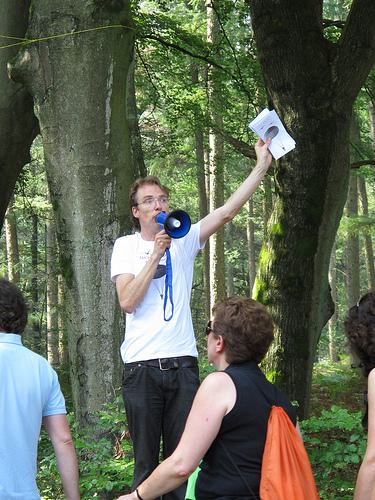
\includegraphics[width=0.11\textwidth]{fig/castream/images/Comparable/figure1_similarities/original/23541.jpeg}&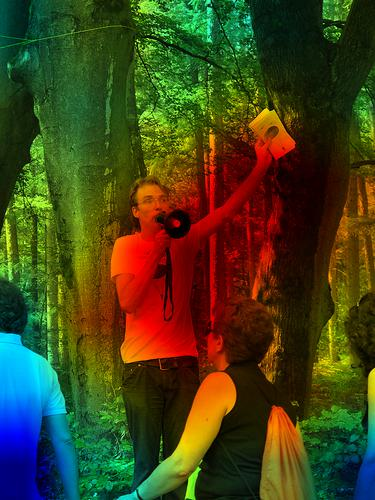
\includegraphics[width=0.11\textwidth]{fig/castream/images/Comparable/figure1_similarities/raw_att/23541.jpeg}&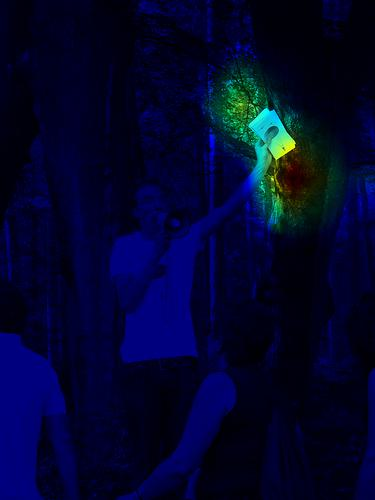
\includegraphics[width=0.11\textwidth]{fig/castream/images/Comparable/figure1_similarities/shelf_gradcam/23541.jpeg}&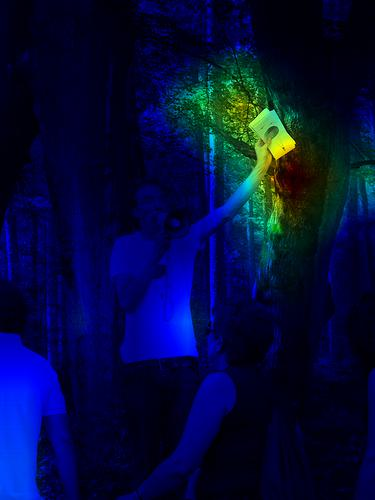
\includegraphics[width=0.11\textwidth]{fig/castream/images/Comparable/figure1_similarities/gradcam/23541.jpeg}&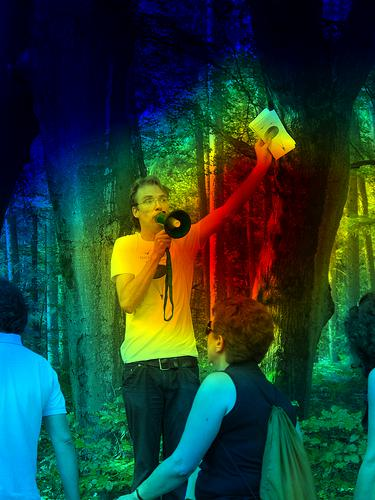
\includegraphics[width=0.11\textwidth]{fig/castream/images/Comparable/figure1_similarities/shelf_gradcampp/23541.jpeg}&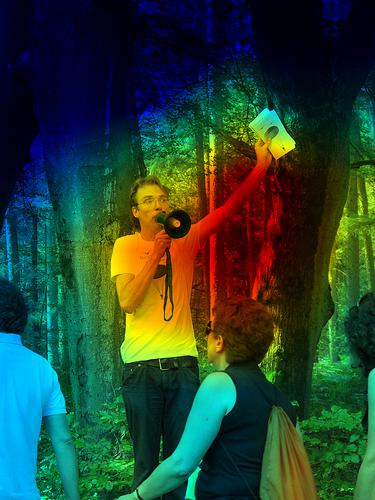
\includegraphics[width=0.11\textwidth]{fig/castream/images/Comparable/figure1_similarities/gradcampp/23541.jpeg}&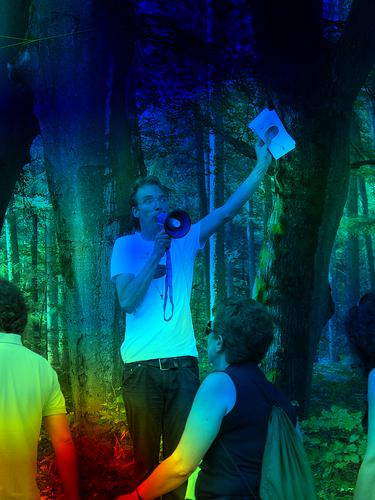
\includegraphics[width=0.11\textwidth]{fig/castream/images/Comparable/figure1_similarities/scorecam/23541.jpeg}&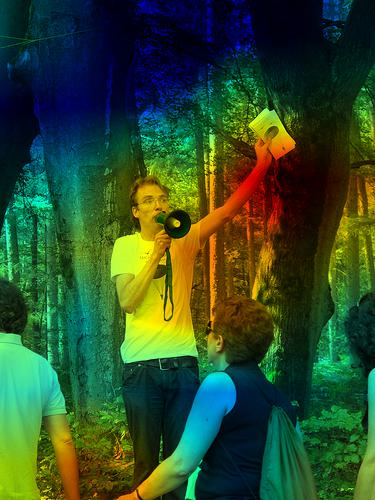
\includegraphics[width=0.11\textwidth]{fig/castream/images/Comparable/figure1_similarities/shelf_scorecam/23541.jpeg}\\
        {\rotatebox{90}{\tiny Groom}}&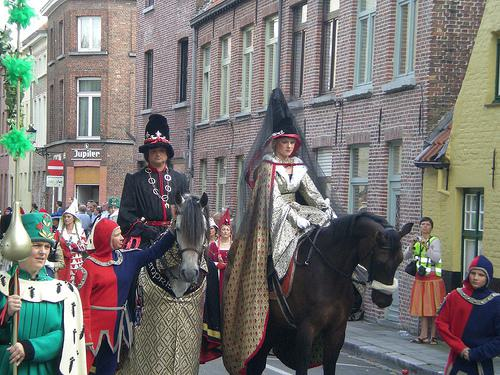
\includegraphics[width=0.11\textwidth]{fig/castream/images/Comparable/figure1_similarities/original/9602.jpeg}&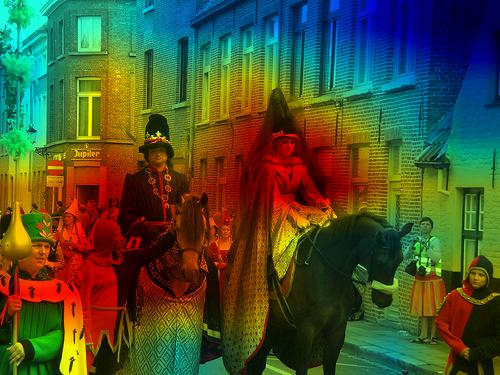
\includegraphics[width=0.11\textwidth]{fig/castream/images/Comparable/figure1_similarities/raw_att/9602.jpeg}&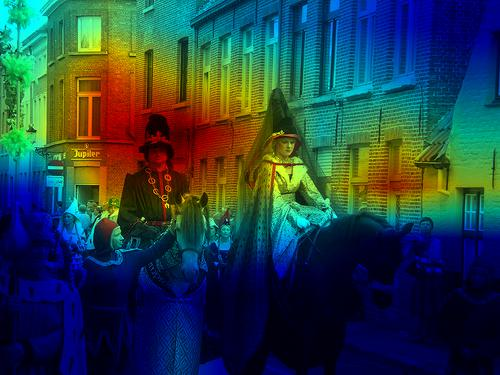
\includegraphics[width=0.11\textwidth]{fig/castream/images/Comparable/figure1_similarities/shelf_gradcam/9602.jpeg}&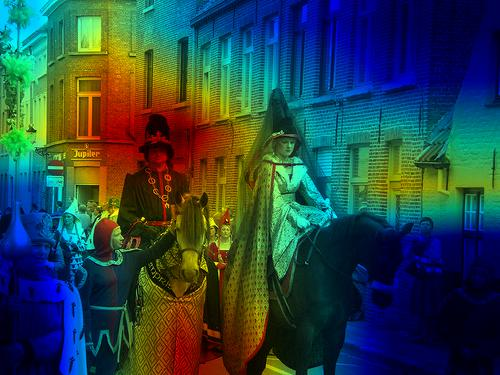
\includegraphics[width=0.11\textwidth]{fig/castream/images/Comparable/figure1_similarities/gradcam/9602.jpeg}&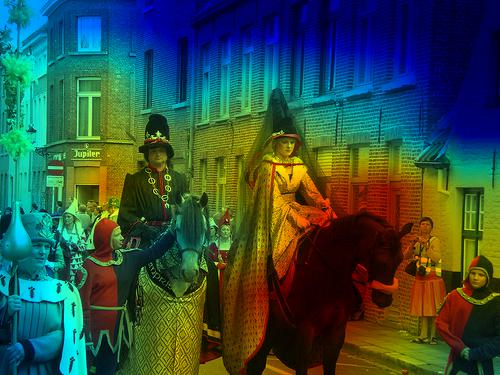
\includegraphics[width=0.11\textwidth]{fig/castream/images/Comparable/figure1_similarities/shelf_gradcampp/9602.jpeg}&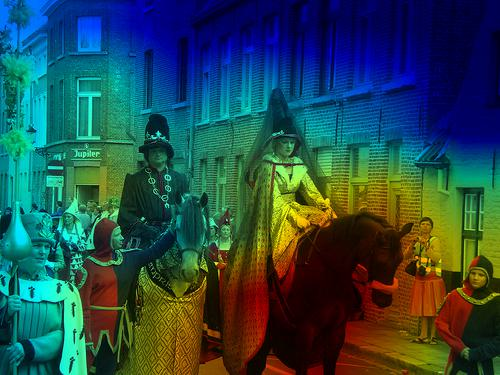
\includegraphics[width=0.11\textwidth]{fig/castream/images/Comparable/figure1_similarities/gradcampp/9602.jpeg}&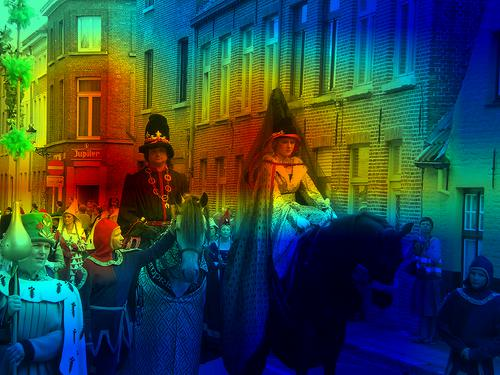
\includegraphics[width=0.11\textwidth]{fig/castream/images/Comparable/figure1_similarities/scorecam/9602.jpeg}&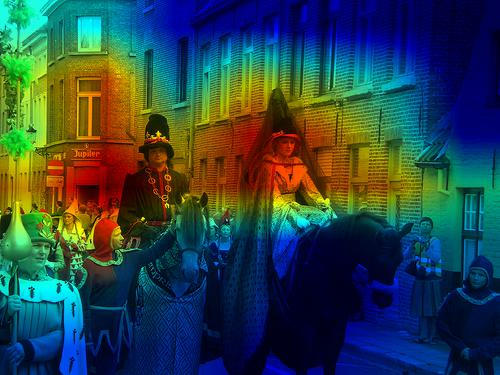
\includegraphics[width=0.11\textwidth]{fig/castream/images/Comparable/figure1_similarities/shelf_scorecam/9602.jpeg}\\    
        {\rotatebox{90}{\tiny Nematode}}&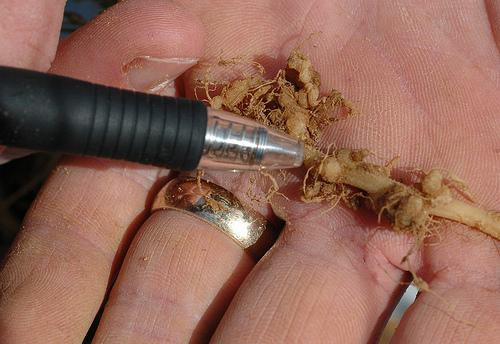
\includegraphics[width=0.11\textwidth]{fig/castream/images/Comparable/figure1_similarities/original/12414.jpeg}&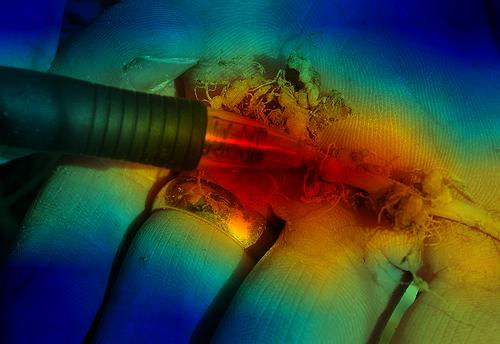
\includegraphics[width=0.11\textwidth]{fig/castream/images/Comparable/figure1_similarities/raw_att/12414.jpeg}&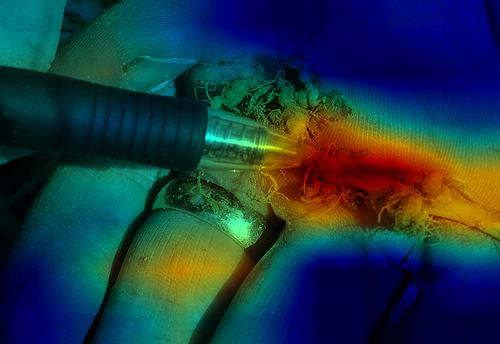
\includegraphics[width=0.11\textwidth]{fig/castream/images/Comparable/figure1_similarities/shelf_gradcam/12414.jpeg}&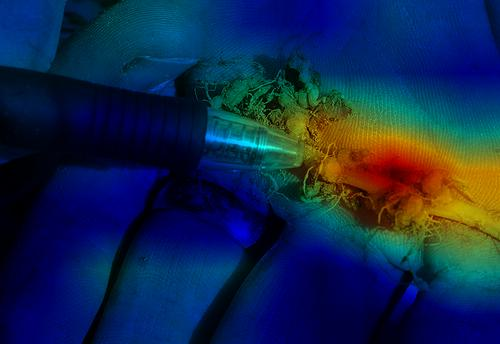
\includegraphics[width=0.11\textwidth]{fig/castream/images/Comparable/figure1_similarities/gradcam/12414.jpeg}&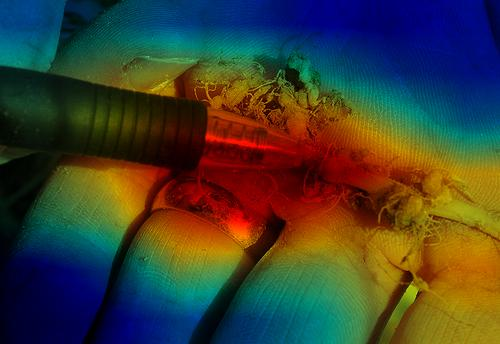
\includegraphics[width=0.11\textwidth]{fig/castream/images/Comparable/figure1_similarities/shelf_gradcampp/12414.jpeg}&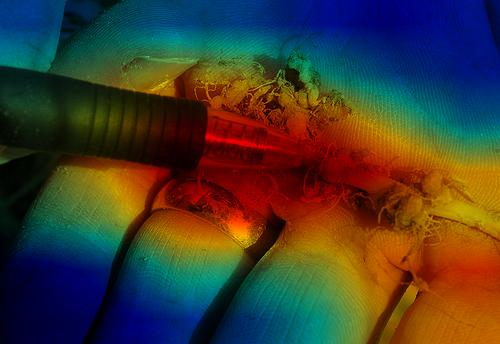
\includegraphics[width=0.11\textwidth]{fig/castream/images/Comparable/figure1_similarities/gradcampp/12414.jpeg}&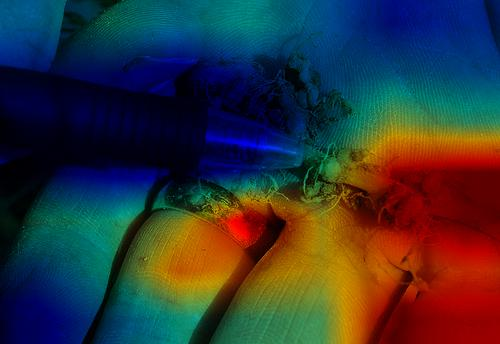
\includegraphics[width=0.11\textwidth]{fig/castream/images/Comparable/figure1_similarities/scorecam/12414.jpeg}&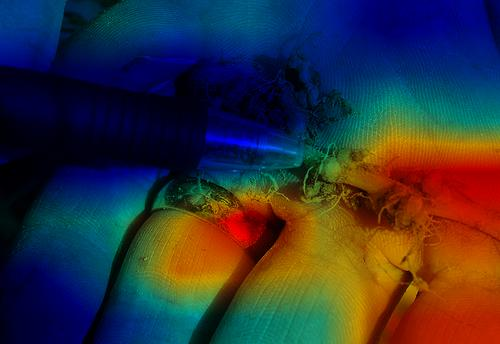
\includegraphics[width=0.11\textwidth]{fig/castream/images/Comparable/figure1_similarities/shelf_scorecam/12414.jpeg}\\
        {\rotatebox{90}{\tiny CRT screen}}&\multicolumn{1}{c}{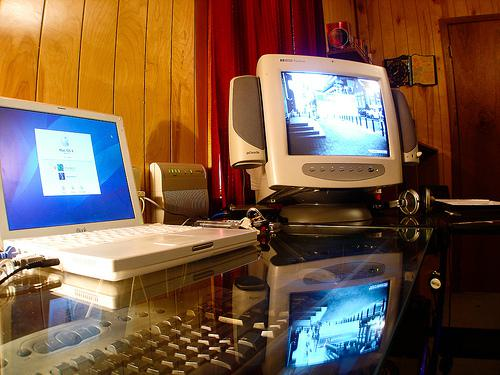
\includegraphics[width=0.11\textwidth]{fig/castream/images/Comparable/figure1/original/43057.jpeg}}&\multicolumn{1}{c}{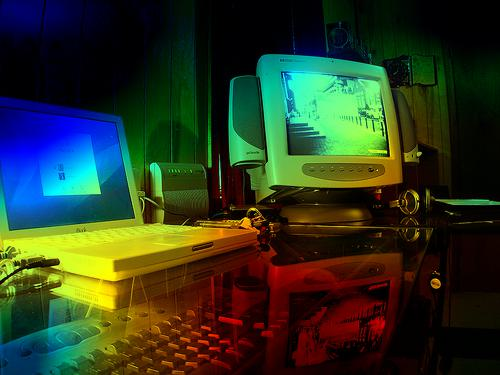
\includegraphics[width=0.11\textwidth]{fig/castream/images/Comparable/figure1/raw_att/43057.jpeg}}&\multicolumn{1}{c}{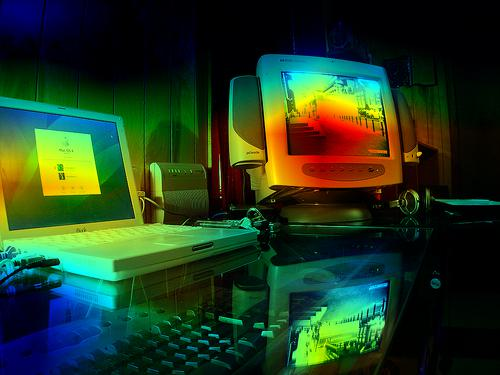
\includegraphics[width=0.11\textwidth]{fig/castream/images/Comparable/figure1/shelf_gradcam/43057.jpeg}}&\multicolumn{1}{c}{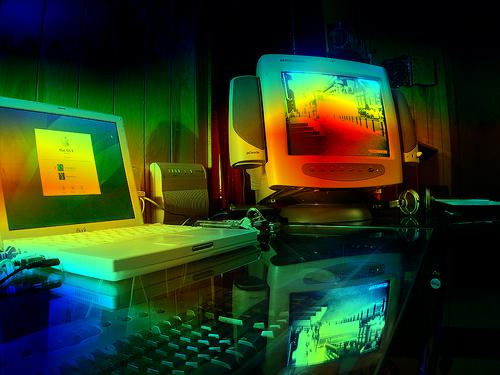
\includegraphics[width=0.11\textwidth]{fig/castream/images/Comparable/figure1/gradcam/43057.jpeg}}&\multicolumn{1}{c}{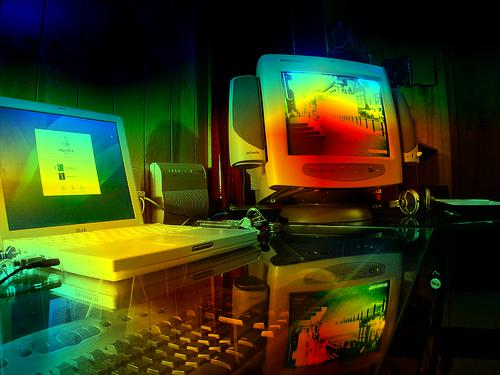
\includegraphics[width=0.11\textwidth]{fig/castream/images/Comparable/figure1/shelf_gradcampp/43057.jpeg}}&\multicolumn{1}{c}{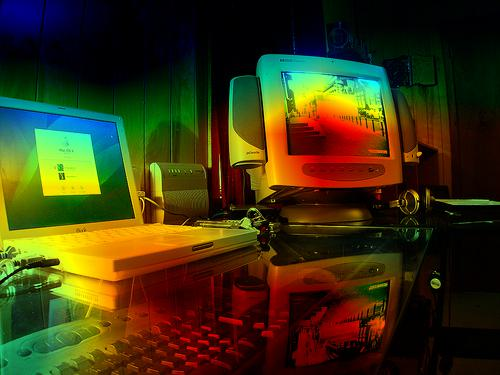
\includegraphics[width=0.11\textwidth]{fig/castream/images/Comparable/figure1/gradcampp/43057.jpeg}}&\multicolumn{1}{c}{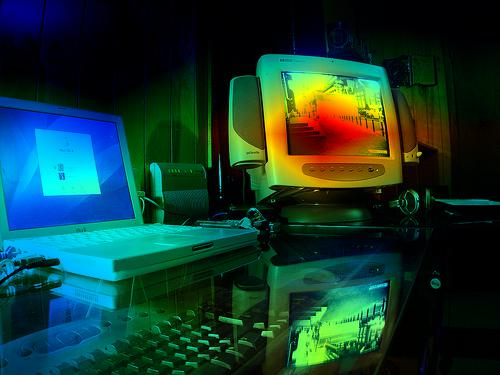
\includegraphics[width=0.11\textwidth]{fig/castream/images/Comparable/figure1/shelf_scorecam/43057.jpeg}}&\multicolumn{1}{c}{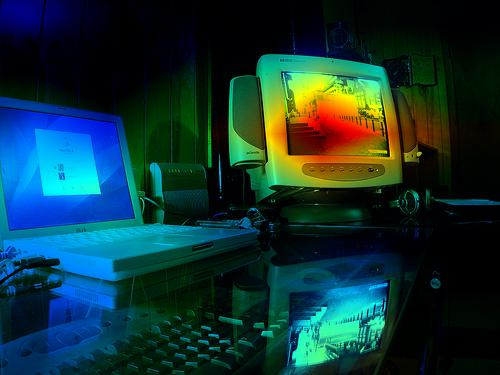
\includegraphics[width=0.11\textwidth]{fig/castream/images/Comparable/figure1/scorecam/43057.jpeg}}\\ % Checked     
        {\rotatebox{90}{\tiny Snowboard}}&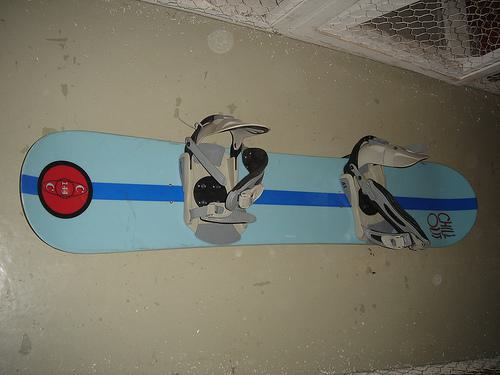
\includegraphics[width=0.11\textwidth]{fig/castream/images/Comparable/figure1_similarities/original/11376.jpeg}&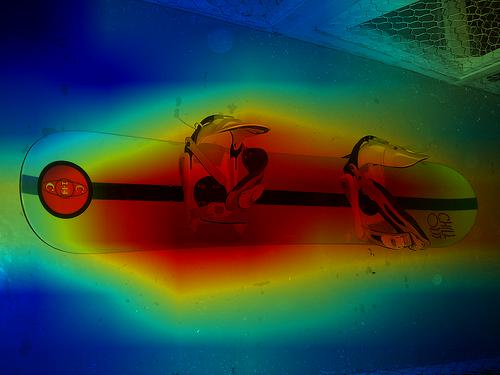
\includegraphics[width=0.11\textwidth]{fig/castream/images/Comparable/figure1_similarities/raw_att/11376.jpeg}&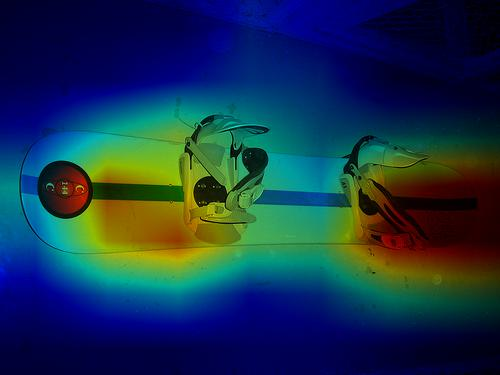
\includegraphics[width=0.11\textwidth]{fig/castream/images/Comparable/figure1_similarities/shelf_gradcam/11376.jpeg}&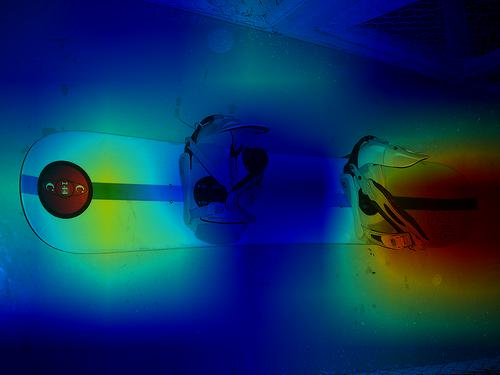
\includegraphics[width=0.11\textwidth]{fig/castream/images/Comparable/figure1_similarities/gradcam/11376.jpeg}&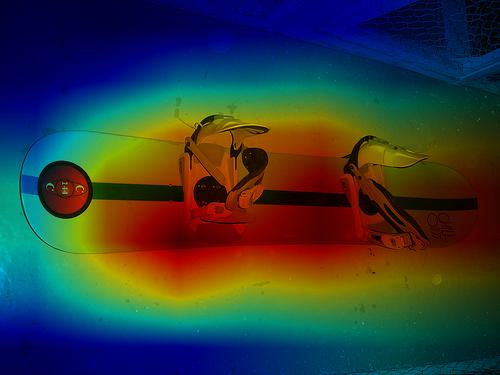
\includegraphics[width=0.11\textwidth]{fig/castream/images/Comparable/figure1_similarities/shelf_gradcampp/11376.jpeg}&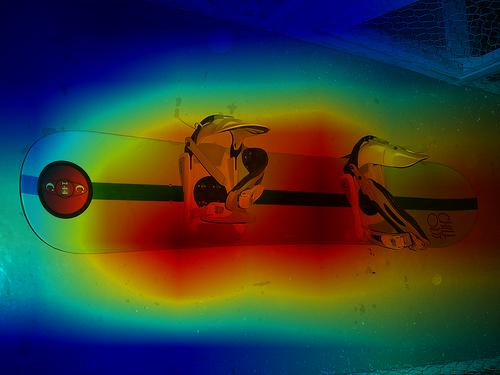
\includegraphics[width=0.11\textwidth]{fig/castream/images/Comparable/figure1_similarities/gradcampp/11376.jpeg}&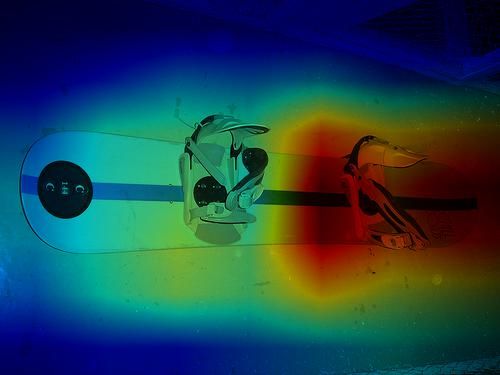
\includegraphics[width=0.11\textwidth]{fig/castream/images/Comparable/figure1_similarities/scorecam/11376.jpeg}&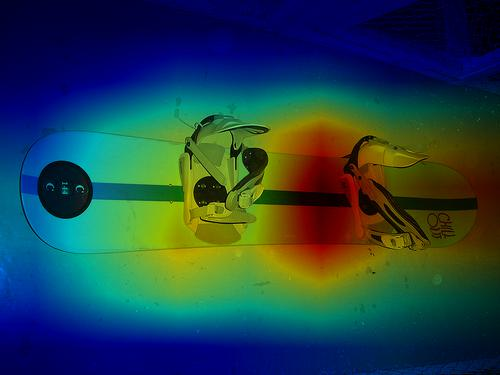
\includegraphics[width=0.11\textwidth]{fig/castream/images/Comparable/figure1_similarities/shelf_scorecam/11376.jpeg}\\   
    \end{tabular}
    % }
    \vspace{3pt}
    \caption{\textbf{Comparison of saliency maps} generated by different CAM-based methods, using GAP and our \Ours, on ImageNet images. The raw attention is the one used for pooling by \Ours.}
    \label{fig:compmethods}
    \end{figure}

\noindent We observe that the raw attention focuses on objects of interest in the images. 
In general, saliency maps obtained with \Ours are similar but tend to cover larger regions of the 
object or more instances compared with \gap.\\
\begin{figure}[t]
\scriptsize
\centering
\setlength{\tabcolsep}{1.3pt}
%    \resizebox{\columnwidth}{!}{%
     \begin{tabular}{cccccccc}
           \mc{2}{Corridor}&\mc{2}{Greenhouse}&\mc{2}{Pool Inside}&\mc{2}{Wine Cellar}\\
           Input image&Raw Attention&Input image&Raw Attention&Input image&Raw Attention&Input image&Raw Attention\\
           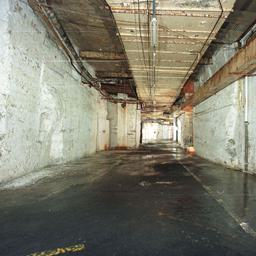
\includegraphics[width=0.12\textwidth,height=0.08\textwidth]{fig/castream/images/Outdataset/Corridor/Original/c1.jpg}&
           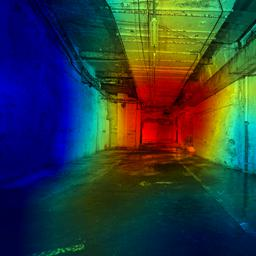
\includegraphics[width=0.12\textwidth,height=0.08\textwidth]{fig/castream/images/Outdataset/Corridor/Attention/c1.jpg}&
           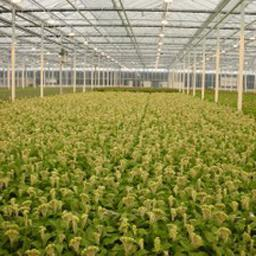
\includegraphics[width=0.12\textwidth,height=0.08\textwidth]{fig/castream/images/Outdataset/Greenhouse/Original/celosie_02.jpg}&
           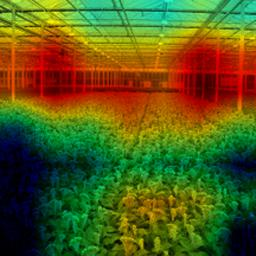
\includegraphics[width=0.12\textwidth,height=0.08\textwidth]{fig/castream/images/Outdataset/Greenhouse/Attention/celosie_02.jpg}&
           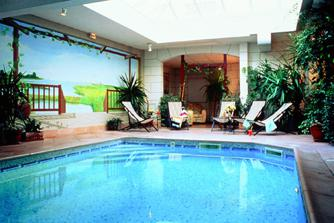
\includegraphics[width=0.12\textwidth,height=0.08\textwidth]{fig/castream/images/Outdataset/Poolinside/Original/003_1b.jpg}&
           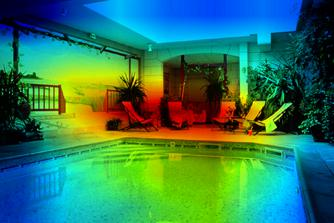
\includegraphics[width=0.12\textwidth,height=0.08\textwidth]{fig/castream/images/Outdataset/Poolinside/Attention/003_1b.jpg}&
           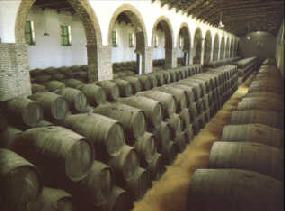
\includegraphics[width=0.12\textwidth,height=0.08\textwidth]{fig/castream/images/Outdataset/WineCellar/Original/bodega2.jpg}&
           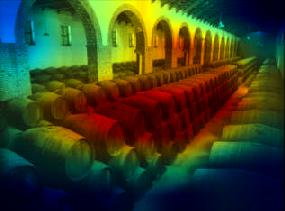
\includegraphics[width=0.12\textwidth,height=0.08\textwidth]{fig/castream/images/Outdataset/WineCellar/Attention/bodega2.jpg}\\
           
           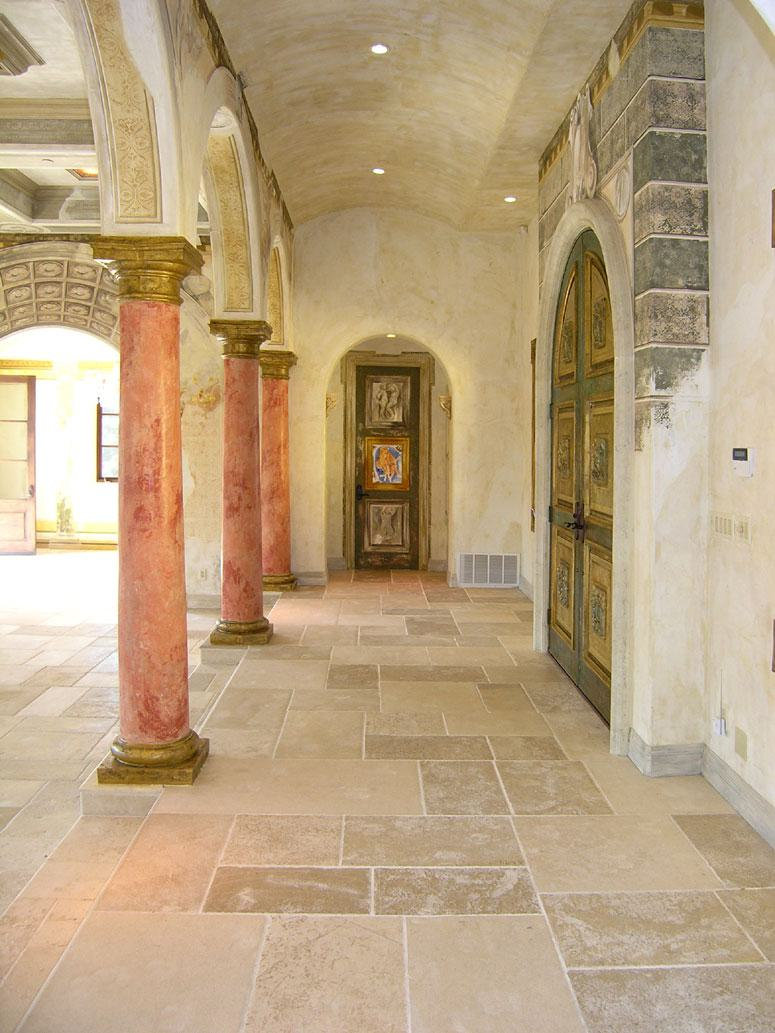
\includegraphics[width=0.12\textwidth,height=0.08\textwidth]{fig/castream/images/Outdataset/Corridor/Original/1L_10_Corridor_A.jpg}&
           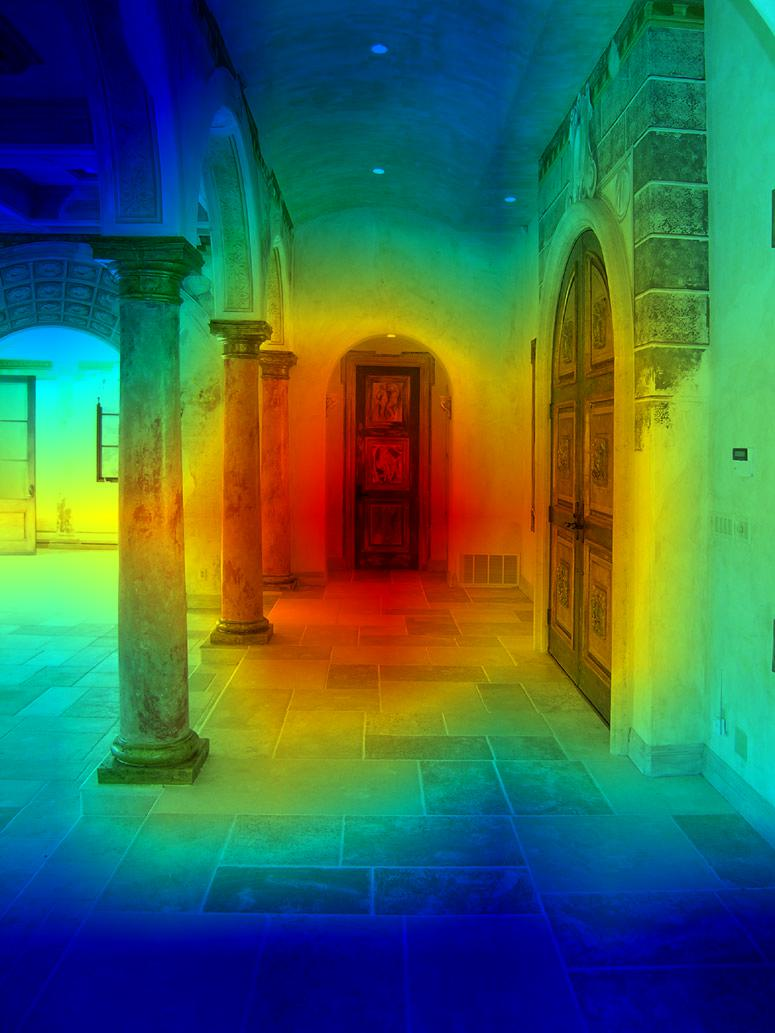
\includegraphics[width=0.12\textwidth,height=0.08\textwidth]{fig/castream/images/Outdataset/Corridor/Attention/1L_10_Corridor_A.jpg}&
           \includegraphics[width=0.12\textwidth,height=0.08\textwidth]{fig/castream/images/Outdataset/Greenhouse/Original/20070417klpcnatun_229_Ies_SCO.jpg}&
           \includegraphics[width=0.12\textwidth,height=0.08\textwidth]{fig/castream/images/Outdataset/Greenhouse/Attention/20070417klpcnatun_229_Ies_SCO.jpg}&
           \includegraphics[width=0.12\textwidth,height=0.08\textwidth]{fig/castream/images/Outdataset/Poolinside/Original/141821195_M.jpg}&
           \includegraphics[width=0.12\textwidth,height=0.08\textwidth]{fig/castream/images/Outdataset/Poolinside/Attention/141821195_M.jpg}&
           \includegraphics[width=0.12\textwidth,height=0.08\textwidth]{fig/castream/images/Outdataset/WineCellar/Original/bodega_45_18_yahoo.jpg}&
           \includegraphics[width=0.12\textwidth,height=0.08\textwidth]{fig/castream/images/Outdataset/WineCellar/Attention/bodega_45_18_yahoo.jpg}\\
           
           \includegraphics[width=0.12\textwidth,height=0.08\textwidth]{fig/castream/images/Outdataset/Corridor/Original/430_Korridor_300.jpg}&
           \includegraphics[width=0.12\textwidth,height=0.08\textwidth]{fig/castream/images/Outdataset/Corridor/Attention/430_Korridor_300.jpg}&
           \includegraphics[width=0.12\textwidth,height=0.08\textwidth]{fig/castream/images/Outdataset/Greenhouse/Original/20070418klpcnaecl_364_Ies_SCO.jpg}&
           \includegraphics[width=0.12\textwidth,height=0.08\textwidth]{fig/castream/images/Outdataset/Greenhouse/Attention/20070418klpcnaecl_364_Ies_SCO.jpg}&
           \includegraphics[width=0.12\textwidth,height=0.08\textwidth]{fig/castream/images/Outdataset/Poolinside/Original/catalogue_piscine_interieur.jpg}&
           \includegraphics[width=0.12\textwidth,height=0.08\textwidth]{fig/castream/images/Outdataset/Poolinside/Attention/catalogue_piscine_interieur.jpg}&
           \includegraphics[width=0.12\textwidth,height=0.08\textwidth]{fig/castream/images/Outdataset/WineCellar/Original/bodega_63_24_flickr.jpg}&
           \includegraphics[width=0.12\textwidth,height=0.08\textwidth]{fig/castream/images/Outdataset/WineCellar/Attention/bodega_63_24_flickr.jpg}\\
           
           \includegraphics[width=0.12\textwidth,height=0.08\textwidth]{fig/castream/images/Outdataset/Corridor/Original/06_Right_corridor_of_the_main_hall.jpg}&
           \includegraphics[width=0.12\textwidth,height=0.08\textwidth]{fig/castream/images/Outdataset/Corridor/Attention/06_Right_corridor_of_the_main_hall.jpg}&
           \includegraphics[width=0.12\textwidth,height=0.08\textwidth]{fig/castream/images/Outdataset/Greenhouse/Original/2026_2006_Grimm_s_Gardens_Greenhouse.jpg}&
           \includegraphics[width=0.12\textwidth,height=0.08\textwidth]{fig/castream/images/Outdataset/Greenhouse/Attention/2026_2006_Grimm_s_Gardens_Greenhouse.jpg}&
           \includegraphics[width=0.12\textwidth,height=0.08\textwidth]{fig/castream/images/Outdataset/Poolinside/Original/connolly_center_pool_inside_lg.jpg}&
           \includegraphics[width=0.12\textwidth,height=0.08\textwidth]{fig/castream/images/Outdataset/Poolinside/Attention/connolly_center_pool_inside_lg.jpg}&
           \includegraphics[width=0.12\textwidth,height=0.08\textwidth]{fig/castream/images/Outdataset/WineCellar/Original/bodega_78_08_flickr.jpg}&
           \includegraphics[width=0.12\textwidth,height=0.08\textwidth]{fig/castream/images/Outdataset/WineCellar/Attention/bodega_78_08_flickr.jpg}\\              
    \end{tabular}
%    }
    \vspace{3pt}
    \caption{\textbf{Raw attention maps} obtained from our \Ours on images of the MIT 67 Scenes dataset \autocite{quattoni2009recognizing} on classes that do not exist in ImageNet. The network sees them at inference for the first time.} 
    %
    \label{fig:enter-label}
\end{figure}  
Indeed, the differences in saliency maps should not be large, as both methods share the same 
features maps $F^k_\ell$ and only the weight coefficients $\alpha^c_k$ differ.
Despite the small differences, the following quantitative results show that \Ours has a significant 
impact on the interpretability metrics.\\
   
\noindent In addition, \autoref{fig:enter-label} shows examples of images from the MIT 67 Scenes 
dataset \autocite{quattoni2009recognizing} along with raw attention maps obtained by \Ours. These 
images come from four classes that do not exist in ImageNet and the network sees them at inference for 
the first time. Nevertheless, the attention maps focus on objects of interest in general.
